\section{Quantum Software Engineering with the Forest SDK}

\subsection{The Forest SDK}

\begin{center}
Info: \url{https://rigetti.com/forest}
\end{center}

The Forest SDK provides a powerful and performant library of tools that are useful in the development of quantum algorithms. Foremost it provides: an optimizing compiler (\verb|quilc|); a quantum virtual machine (\verb|qvm|) for prototyping and debugging; and a Python-based interface to the Quantum Cloud Services (QCS) stack. To install the Forest SDK, follow the URL appropriate for your computer:
\begin{itemize}
    \item macOS: \href{https://downloads.rigetti.com/qcs-sdk/forest-sdk.dmg}{\underline{dmg installer}}
    \item Linux-based: \href{https://downloads.rigetti.com/qcs-sdk/forest-sdk-linux-deb.tar.bz2}{\underline{deb installer}} or \href{https://downloads.rigetti.com/qcs-sdk/forest-sdk-linux-barebones.tar.bz2}{\underline{barebones tarball}}
    \item Windows: \href{https://downloads.rigetti.com/qcs-sdk/forest-sdk.msi}{\underline{msi installer}}
\end{itemize}
Finally install pyQuil with either
\begin{bash}
pip install pyquil==2.7.2
\end{bash}
or
\begin{bash}
conda install -c rigetti pyquil==2.7.2
\end{bash}

\subsection{The Quil Compiler}
\begin{center}
Source Code: \url{https://github.com/rigetti/quilc/}
\end{center}

Quantum programs that are intended to be run on Rigetti QPUs are specified in the assembly-like Quil. While Quil is somewhat low-level it provides methods of abstraction. For example, the base language provides you with many of the gates commonly seen in the literature (e.g. \Hadamard{}, \CNOT{}). Quil's \verb|DEFGATE| allows us to define new gates, by providing a name and some unitary matrix. We also frequently find it helpful to think in terms of circuits---collections of gate applications. Quil provides \verb|DEFCIRCUIT| for this case.

It is ultimately expected that our Quil programs will be executed on a QPU. However, the gates that a QPU understands are typically very limited---this small set of supported gates is called the native gateset of the QPU. Rigetti's native gateset includes just three 1Q gates $\RX(\pm\pi/2)$ and $\RZ(\alpha)$ as well as one 2Q gate \CZ{}. (It is an incredible result of quantum computing research that just these three gates can produce any arbitrary unitary gate---they are universal). 

This presents a problem: Quil the language provides gates not in the native gateset, and further it provides ways to create new gates, also not in the native gateset! And all this with the expectation that it can be run on a QPU. We might just require that Quil programs target the native gateset and be done with it, but that's no fun for anyone. Methods of abstraction make for a powerful and expressive language. Instead we offload this overhead to the compiler: we provide quilc with an arbitrary Quil program and some description of the architecture that we want to target called the ISA. (Technically the ISA encompasses more than just the native gateset: we can include information about the topology and specifications of the available qubits.) The compiler then produces Quil code that targets the specified ISA.

Fortunately the compiler isn't tied to just the Rigetti architecture. In fact it has support for various architectures including Google's 72Q ``Bristlecone'' device, and IBM's 16Q ``ibmqx5'' device. These are ISAs that are hard-coded into the compiler, but implementing a new ISA is mostly as simple as writing out a JSON file and giving it to the compiler.

The compiler does an awful lot more than just mechanically translate non-gateset instructions to gateset instructions. It applies numerous optimization routines, determines resource usage amongst instructions, decomposes complex unitary matrices into smaller and smaller square matrices. All with the intent that the resulting program is equivalent to---but more efficient than---the input program.\footnote{There are unfortunate cases where the compiler does a poor job and ends up producing unnecessarily complex programs. But that's good---we have problems to keep us employed.}

After installing \verb|quilc| you can send it input directly through the command line. For example compile a Hadamard gate on qubit zero:
\begin{bash}
echo "H 0" | quilc

RZ(pi/2) 0                  # Entering rewiring: #(0 1 2 3 4 5 6 7)
RX(pi/2) 0
RZ(pi/2) 0
HALT                        # Exiting rewiring: #(0 1 2 3 4 5 6 7)
\end{bash}
As expected, the compiler has translated the non-native gate \verb|H 0| into a sequence of native gates.

If your program is longer, we can separate them with newlines. This requires the \verb|-e| option to \verb|echo|:
\begin{bash}
echo "H 0\nH 1" | quilc

RZ(pi/2) 0                  # Entering rewiring: #(0 1 2 3 4 5 6 7)
RX(pi/2) 0
RZ(pi/2) 0
RZ(pi/2) 1
RX(pi/2) 1
RZ(pi/2) 1
HALT                        # Exiting rewiring: #(0 1 2 3 4 5 6 7)
\end{bash}

If the command line is getting too unweildy, we can write the same program in a file, say \verb|super.quil|:
\begin{quil}
H 0
H 1
\end{quil}
and then we can \verb|cat| this file into the compiler: \verb/cat super.quil | quilc/.

Try the following and reason about the results:
\begin{itemize}
\item Consecutive Hadamards on the same qubit.
\item Two \verb|H| on the same qubit sandwiching a \verb|H| on a different qubit.
\item Two \verb|H| on the same qubit, sandwiching a \verb|CNOT| on the same qubits.
\end{itemize}

See \verb|quilc --help| for options to configure the compiler. What happens if you use \verb|quilc --isa ibmqx5| for the above?

\subsection{The QVM}
\begin{center}
Source Code: \url{http://github.com/rigetti/qvm}
\end{center}

QPUs are a scarce resource. They are expensive. And noisy. And don't have many qubits. Think about the early days of classical computing---those computers, UNIVAC, ENIAC, etc.\ filled rooms. They were programmed with switches or punched cards, and those programs were debugged by the same process many of us write code today---try it and see. Except back then \emph{try it and see} might mean \emph{wait until tomorrow for the results} followed by \emph{explain to your supervisor why you wasted hours of compute time and \$\$\$ because of a misplaced semi-colon}.

QPUs of today are somewhat like those old big goofy computers. But today we have much better technology to support that scarce resource. We have the modern internet and all the cool stuff that it supports, so that we can share QPU resources pretty efficiently over the network. But at a more immediate level, we can retain the feel of rapid prototyping of code by targeting a quantum virtual machine (QVM).

The spooky probabilistic essence of quantum mechanics can be simulated on classical computers. While the results are \emph{not} obtained by truly quantum means, and the classical resource usage does not scale too nicely\footnote{The wavefunction of $n$ qubits is a $2^n$-length array of complex coefficients. The memory required for a 26-qubit simulation is of order 1~GB; for 36 qubits, 1~TB. You see the unfortunate situation.}, the behaviour and evolution of the wavefunction are approximated well-enough. The upshot of the above is that with reasonably powerful computers (laptops will generally do fine for low numbers of qubits, around $26$) we can enjoy the rapid prototype-feedback loop that we take for granted when developing algorithms for classical computers.

To get a feel of the QVM, you can interact with it directly on the command line (as with \verb|quilc|). The QVM takes as input some Quil code, and then will return to you the final state of the wavefunction. For example, let's investigate how \verb|H 0| changes the state of the wavefunction:
\begin{bash}
echo "H 0" | qvm --quiet

Classical memory (low -> high indexes):
    No memory.
Amplitudes:
    |0>: 0.7071067811865475,                                    P= 50.0%
    |1>: 0.7071067811865475,                                    P= 50.0%
\end{bash}
The wavefunction is in an equal superposition of $\ket{0}$ and $\ket{1}$. As with \verb|quilc|, you can use the \verb|-e| option to \verb|echo| or use \verb|cat|.

With the QVM, explore and reason about the wavefunction in the following situations:
\begin{itemize}
    \item Flip a single arbitrary bit in the ket. Flipping the $k$\textsuperscript{th} bit has a state that can be written $\ket{2^k}$. For example, flipping the third bit would be $\ket{2^3}=\ket{1000}$.
    \item Construct a Bell state: $\tfrac{1}{\sqrt{2}}(\ket{00}+\ket{11})$.
    \item Construct a GHZ state on 6 qubits: $\tfrac{1}{\sqrt{2}}(\ket{000000}+\ket{111111})$.
    \item Explain why it seems that operators sometimes do nothing.
    \begin{itemize}
        \item We start off in the $\ket{000\ldots00}$ state, and a $\PauliZ$ appears to do nothing. Why?
        \item First put the system in uniform superposition by computing the $\Hadamard$ gate on each qubit. Provide intuition as to why doing any $\PauliX$ gate on any qubit leaves the system unchanged.
    \end{itemize}
\end{itemize}

\subsection{Writing Quil with pyQuil}
\begin{center}
Source Code: \url{https://github.com/rigetti/pyquil}

Documentation: \url{https://pyquil.readthedocs.io/}
\end{center}

Quil is by design simple. It is helpful to think of Quil as an intermediate language (IL) that is produced by some high-level language like Python, and is consumed by the compiler. The simplicity of Quil reduces the complexity of the compiler, and having a high-level language like Python provides the developer with a familiar environment and access to all Python's libraries (e.g. numpy). pyQuil was developed with this goal in mind.

The fundamental objects in pyQuil are:
\begin{description}
\item[\texttt{Program}] This class holds a representation of a program that, when the time is right, will output as text Quil code that can be sent off to the compiler, the simulator, the QPU, etc.
\begin{python}
from pyquil import Program
\end{python}
\item[\texttt{Gate}] All of your favourite gates are defined within pyQuil, e.g. \texttt{H}, \texttt{CNOT}, \texttt{CPHASE}, etc. 
\begin{python}
from pyquil.gates import *
\end{python}
\item[\texttt{QuantumComputer}] This class encapsulates the interface to running Quil code. This object is backed primarily by a compiler object \texttt{QuantumComputer.compiler} and a QAM-implementing object \texttt{QuantumComputer.qam}. The actual behaviour of these depends on your use-case: for example, if you are targeting the QVM, then \texttt{QuantumComputer.qam} will be a \texttt{QVM} object that knows how to call out to the QVM server. Likewise for QPU.
\begin{python}
from pyquil import get_qc
\end{python}
\end{description}

The general progression of programming in pyQuil is:
\begin{enumerate}
\item Write your quantum program in terms of gates, defining new gates where you need them;
\item Call \verb|pyquil.get_qc()| to get your \verb|QuantumComputer| object. 

The first argument to \verb|pyquil.get_qc()| is a string that describes the device you would like to target, and at first the syntax can seem strange. If you're targeting a QPU, then the string will be the name of the device and lattice. For example, if you had booked time on \emph{Aspen-3}'s \emph{8Q-A} lattice, then you would use
\begin{python} 
qc = pyquil.get_qc('Aspen-3-8Q-A')
\end{python}
If you simply want to target a QVM with the same device ISA, you can append the string ``-qvm'' to the device name
\begin{python}
qc = pyquil.get_qc('Aspen-3-8Q-A-qvm')
\end{python}

During exploration, a commonly-used device name is ``8q-qvm'' which gives you a QVM with a connected graph of eight qubits---any pair of qubits has a connecting edge, and thus can occur in a two-qubit gate (very unphysical). You can even design your own device with a novel graph if you'd like: see \verb|pyquil.api._quantum_computer._get_qvm_with_topology|.
\item Your \verb|qc| object now furnishes you with some methods for running a program. Maybe the most interesting of which are the creatively (and confusingly) named \verb|qc.run()| and \verb|qc.run_and_measure()|.
\end{enumerate}

Let's try a quick example of constructing a Bell state on a QVM and reading out the state.

\begin{python}
from pyquil import Program, get_qc
from pyquil.gates import *

p = Program(H(0), CNOT(0, 1))
qc = get_qc('2q-qvm')

print(qc.run_and_measure(p, trials=10))
\end{python}

And as expected we see entanglement!

\begin{python}
{0: array([0, 1, 1, 1, 1, 0, 1, 1, 0, 1]), 
 1: array([0, 1, 1, 1, 1, 0, 1, 1, 0, 1])}
\end{python}

For fun, try the above \verb|quilc| and \verb|qvm| exercises from within pyQuil.

\subsection{Implementing QFT with pyQuil}

Rather than give a lecture on the technical details of the Quantum Fourier Transform, I will instead leave that to more educated folks and focus on the implementation of a 3Q QFT\footnote{For those that would like some light reading on the subject, see \cite{qft}.} in pyQuil. On the Fourier transform I will simply say this: we can compute the frequencies that make up a signal. And also this: it is very cool.

\begin{figure}
    \centering
    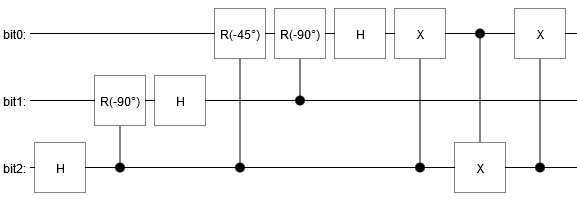
\includegraphics[width=0.8\linewidth]{qft.png}
    \caption{A circuit implementing a 3Q QFT. (Image courtesy \cite{qft})}
    \label{fig:qft}
\end{figure}

There is a well-known circuit that implements the QFT, and we show a 3Q version in fig.~\ref{fig:qft}. Once we identify that the controlled \verb|R| gates correspond to \verb|CPHASE| gates, then we can quite quickly supply the equivalent\footnote{You may notice a difference: our program uses a SWAP gate apparently not present in the original. Why do you think that is?} pyQuil program:
\begin{python}
from pyquil import Program
from pyquil.gates import *
from math import pi

qft = Program(
    SWAP(0, 2),
    H(0),
    CPHASE(-pi / 2.0, 0, 1),
    H(q1),
    CPHASE(-pi / 4.0, 0, 2),
    CPHASE(-pi / 2.0, 1, 2),
    H(2))
\end{python}

We now prepare our desired initial state. This can often be a difficult task\footnote{If you're feeling particularly peppy, have a bash at creating a $W$-state: $\tfrac{1}{\sqrt{3}}(\ket{001}+\ket{010}+\ket{100})$.}, so we'll stick to a simple initial state of $\ket{010}$
\begin{python}
initial_state = Program(I(0), X(1), I(2))
\end{python}
We need the identity gates in order to force the simulator to use three qubits. Without them, the QVM will try to optimize the program into a one-qubit one.

Almost there. Now we need a QVM to run this stuff for us. We really want access to the wavefunction amplitudes as it evolves since this is where the frequencies of the QFT will be encoded. Unfortunately this is a big no-no in quantum mechanics. Nevertheless, since we have a simulator that simulates quantum mechanics, we can pick and choose how strict we want our quantum mechanics to be: the \verb|WavefunctionSimulator| gives us enough information, and evolves the state as expected.

\begin{python}
from pyquil.api import WavefunctionSimulator

wf_sim = WavefunctionSimulator()
wf = wf_sim.wavefunction(initial_state)
print(wf)
\end{python}

$\ket{010}$ as expected. Now our program in full needs to consist of the state preparation and the QFT program

\begin{python}
prog = initial_state + qft
\end{python}

We're now ready to call out to the QVM and see where this thing takes us! Strap in.

\begin{python}
wavefunction = wf_sim.wavefunction(prog)
print(wave_function.pretty_print())
\end{python}

The result of which is 
\begin{python}
(0.35+0j)|000> + -0.35j|001> 
+ (-0.35+0j)|010> + 0.35j|011> 
+ (0.35+0j)|100> + -0.35j|101> 
+ (-0.35+0j)|110> + 0.35j|111>
\end{python}
It's not immediately obvious that this is the correct result. We can however at this point lean on the \emph{inverse} Fourier transform to confirm our hopes:

\begin{python}
from numpy.fft import ifft
wf = ifft(wavefunction.amplitudes, norm="ortho")
\end{python}

The result of which, is, again somewhat unconvincing:

\begin{python}
array([0.+0.000000e+00j, 0.+0.000000e+00j, 1.+3.061617e-17j,
       0.+0.000000e+00j, 0.+0.000000e+00j, 0.+0.000000e+00j,
       0.-3.061617e-17j, 0.+0.000000e+00j])
\end{python}

Squinting for a moment, you will notice that all but one of these entries are zero (or close enough) and we are thus left with the state $\ket{010}$. We can demonstrate that by printing the wavefunction

\begin{python}
from pyquil.wavefunction import Wavefunction
print(Wavefunction(amplitude_vector=wf)
\end{python}